% !TeX spellcheck = es_MX-SpanishMexico
%----------------------------------------------------------------------------------------------------
%                           		  ENTRE LÍNEAS DE TIERRA

% Curso: Arqueología Bíblica
% Módulo 1: Introducción, Definiciones y Conceptos
% Elabora: Rodrigo Gerardo Trejo Arriaga

%----------------------------------------------------------------------------------------------------

% FORMATO DEL DOCUMENTO


\documentclass[11pt]{article} % Letra estandar

\usepackage[utf8]{inputenc}

%\usepackage{tgadventor}
%\renewcommand{\familydefault}{\sfdefault}

\usepackage[light,math]{iwona}

\usepackage[T1]{fontenc}


\usepackage[spanish]{babel}
\addto\captionsspanish{\renewcommand{\abstractname}{\large{Introducción}}}

\usepackage[margin=1in,letterpaper]{geometry}

\usepackage{fancyhdr} % Paquete para personalizar encabezado y pie de página
\pagestyle{fancy} % Establece que personalizaremos el pie de pagina y el encabezado
\setlength{\headheight}{13.59999pt} % Establece la altura del encabezado
\fancyhead[R]{\textcolor{darkBlue}{Teoría de la Computación}} % Encabezado derecho
\fancyhead[L]{\textit{\textcolor{darkBlue}{Escuela Superior de Cómputo}}} % Encabezado izquierdo
\fancyfoot[L]{\textit{\textcolor{darkBlue}{Práctica 1}}} % Pie de página izquierdo 
\fancyfoot[R]{\textcolor{darkBlue}{\thepage}} % Pie de página  derecho
\fancyfoot[C]{} % Elimina la nueración central de páginas en el pie de página
\renewcommand{\headrulewidth}{0.5pt} % Grosor de la linea de encabezado
\renewcommand{\footrulewidth}{0.5pt} % Grosor de la linea de pie de página

\usepackage{enumitem}

\usepackage{changepage}

\usepackage{graphicx}

\usepackage{tabularx}

\setlength{\parskip}{8pt}

\usepackage{xcolor}
\definecolor{darkBlue}{rgb}{0,0,0.31}
%\definecolor{darkBlue}{rgb}{0,0,0.5}
\definecolor{munsell}{rgb}{0.0, 0.5, 0.69}
\definecolor{indigo}{rgb}{0.0, 0.25, 0.42}
\renewcommand{\footrulewidth}{2pt}
\renewcommand{\footrule}{\hbox to\headwidth{\color{darkBlue}\leaders\hrule height \footrulewidth\hfill}}

\usepackage{colortbl}

\usepackage{titlesec}
\titleformat{\section}
{\normalfont\Large\bfseries\color{darkBlue}}{\thesection.}{1em}{}

\usepackage{tabularx}

\usepackage{textcomp}

\usepackage{titling}

\usepackage{apacite}
\bibliographystyle{apacite}

%\usepackage{natbib}
%\setlength{\bibsep}{6pt}

\usepackage{setspace}

\usepackage{listings}


\lstset{
	language=Python,                % Lenguaje del código (Python en este caso)
	basicstyle=\ttfamily,           % Estilo de fuente
	keywordstyle=\color{blue},      % Estilo para las palabras clave
	commentstyle=\color{green},     % Estilo para los comentarios
	numbers=left,                   % Colocar números de línea a la izquierda
	numberstyle=\tiny\color{gray},  % Estilo para los números de línea
	stepnumber=1,                   % Número de línea cada 1 línea
	tabsize=4,                      % Tamaño de la tabulación
	frame=single,                   % Colocar un marco alrededor del código
	breaklines=true,                % Romper líneas largas automáticamente
	showstringspaces=false,         % No mostrar espacios en cadenas
	escapeinside={(*@}{@*)},        % Para incluir caracteres especiales en el código
	extendedchars=true               % Permitir caracteres especiales, como acentos
}


\renewcommand{\thesection}{\Roman{section}}

%----------------------------------------------------------------------------------------------------
% CUERPO DEL DOCUMENTO

\begin{document}
	
	\begin{titlepage}
		\centering
		{
\includegraphics[width=0.25\textwidth]{descarga}\par}
		\vspace{0.5cm}
		{\bfseries\huge Escuela Superior de Cómputo \par}
		\vspace{0.7cm}
		{\scshape\LARGE Teoría de la Computación \par}
		\vspace{0.3cm}
		\vspace{3.1cm}
		{\scshape \Huge \textbf{Práctica 1:}  \par}
		\vspace{0.03cm}
		{{\LARGE \textit{Universo}} \par}
		%\vfill
		\vspace{3.5cm}
		{\Large Autor: \par}
		{\Large Rodrigo Gerardo Trejo Arriaga \par}
		%\vfill
		\vspace{3cm}
		{\Large Octubre 2023 \par}
	\end{titlepage}
	
	\begin{center}
		\vspace*{0.1cm}
		{\huge \textcolor{darkBlue}{\textbf{Práctica 1:}} \par}
		
		{\Large \textcolor{darkBlue}{\textbf{\textit{Universo}}}}
	\end{center}
	
	En la teoría de la computación, un alfabeto se define como un conjunto finito de símbolos o caracteres. Estos símbolos son la base fundamental para construir cadenas o secuencias de símbolos. Por ejemplo, en el contexto de la teoría de la computación, es común utilizar el alfabeto ${0, 1}$ para representar símbolos binarios.
	
	Una cadena, también conocida como palabra, es una secuencia finita de símbolos tomados de un alfabeto dado. Estas cadenas desempeñan un papel esencial en la representación de datos y forman la base de los lenguajes formales en la teoría de la computación.
	
	El conjunto universo, por otro lado, hace referencia a un conjunto que contiene todos los objetos posibles que son relevantes para un problema o lenguaje específico. Por ejemplo, si se trata de un lenguaje de programación, el conjunto universo podría consistir en todos los programas concebibles que se pueden escribir en ese lenguaje.
	
	En el contexto de la teoría de la computación, un lenguaje formal se define como un conjunto de cadenas (palabras) construidas a partir de un alfabeto dado. Estos lenguajes formales se utilizan para describir propiedades de las cadenas y son fundamentales en la definición de gramáticas formales, autómatas y en la resolución de diversos problemas relacionados con la informática teórica.
	
	En esta práctica presentaremos un programa que conjunta todos estos conceptos.
	
	\section{Descripción del problema}
	
	Este programa calcula el universo de cadenas binarias ($\Sigma^n$), donde "n" es un valor determinado por el usuario o calculado automáticamente por el programa. El rango de "n" está restringido al intervalo [0, 1000].
	
	\begin{enumerate}
		\item Ejecute el programa y especifique el valor de "n" que desea calcular.
		\item El programa preguntará si desea calcular otro valor de "n" o salir.
		\item Los resultados se guardarán en un archivo de texto en notación de conjunto.
		\item A continuación, graficaremos el número de unos en cada cadena. El eje "x" representa las cadenas y el eje "y" representa el número de unos en cada cadena.
		\item En el informe, se explicará, calculará y graficará el caso específico en el que "n=28".
		\item Además, se calculará una segunda gráfica utilizando el logaritmo en base 10 del número de unos.
	\end{enumerate}
	
	
	\section{Resultados}
	
	
	
	\begin{figure}[h]
		\centering
		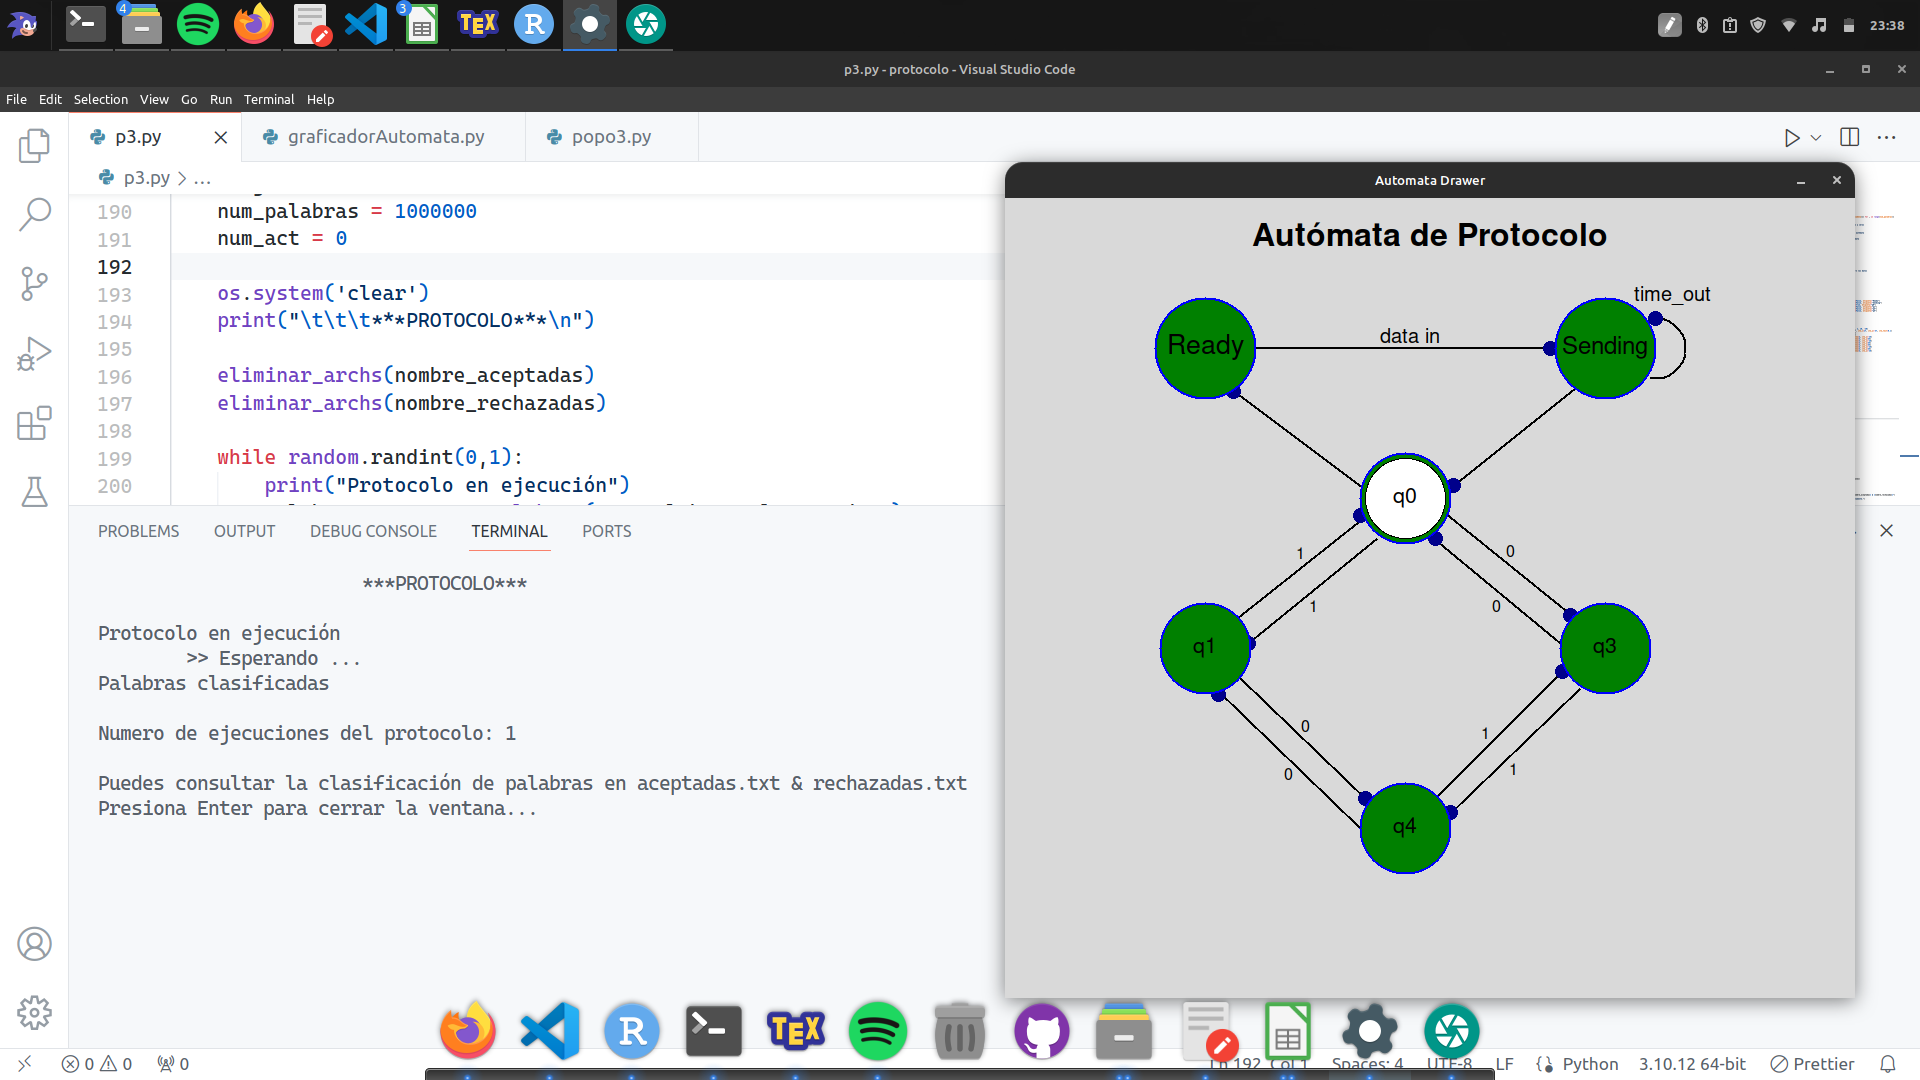
\includegraphics[width=0.8\textwidth]{imagen1.png}
		\caption{Protocolo con su autómata}
	\end{figure}
	
	\begin{figure}[h]
		\centering
		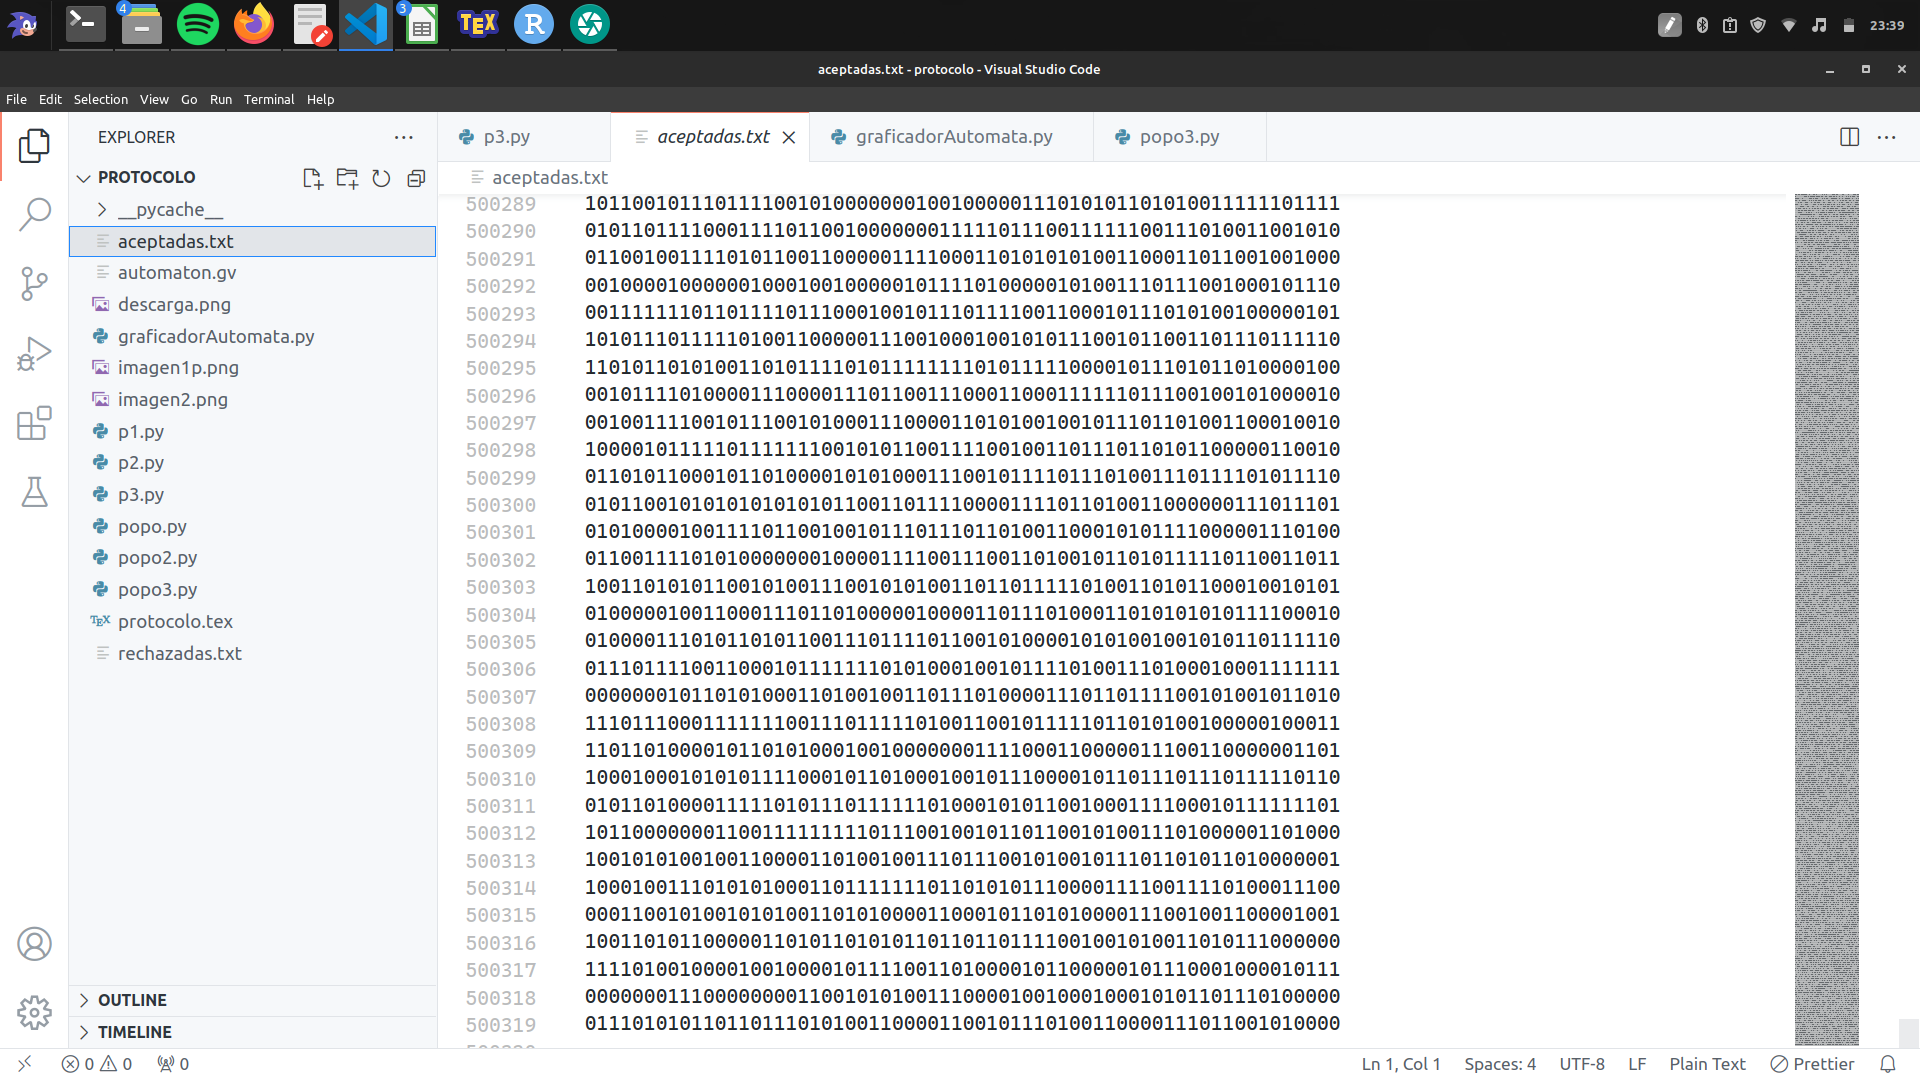
\includegraphics[width=0.8\textwidth]{imagen2.png}
		\caption{Archivo de aceptadas}
	\end{figure}
	
	\begin{figure}[h]
		\centering
		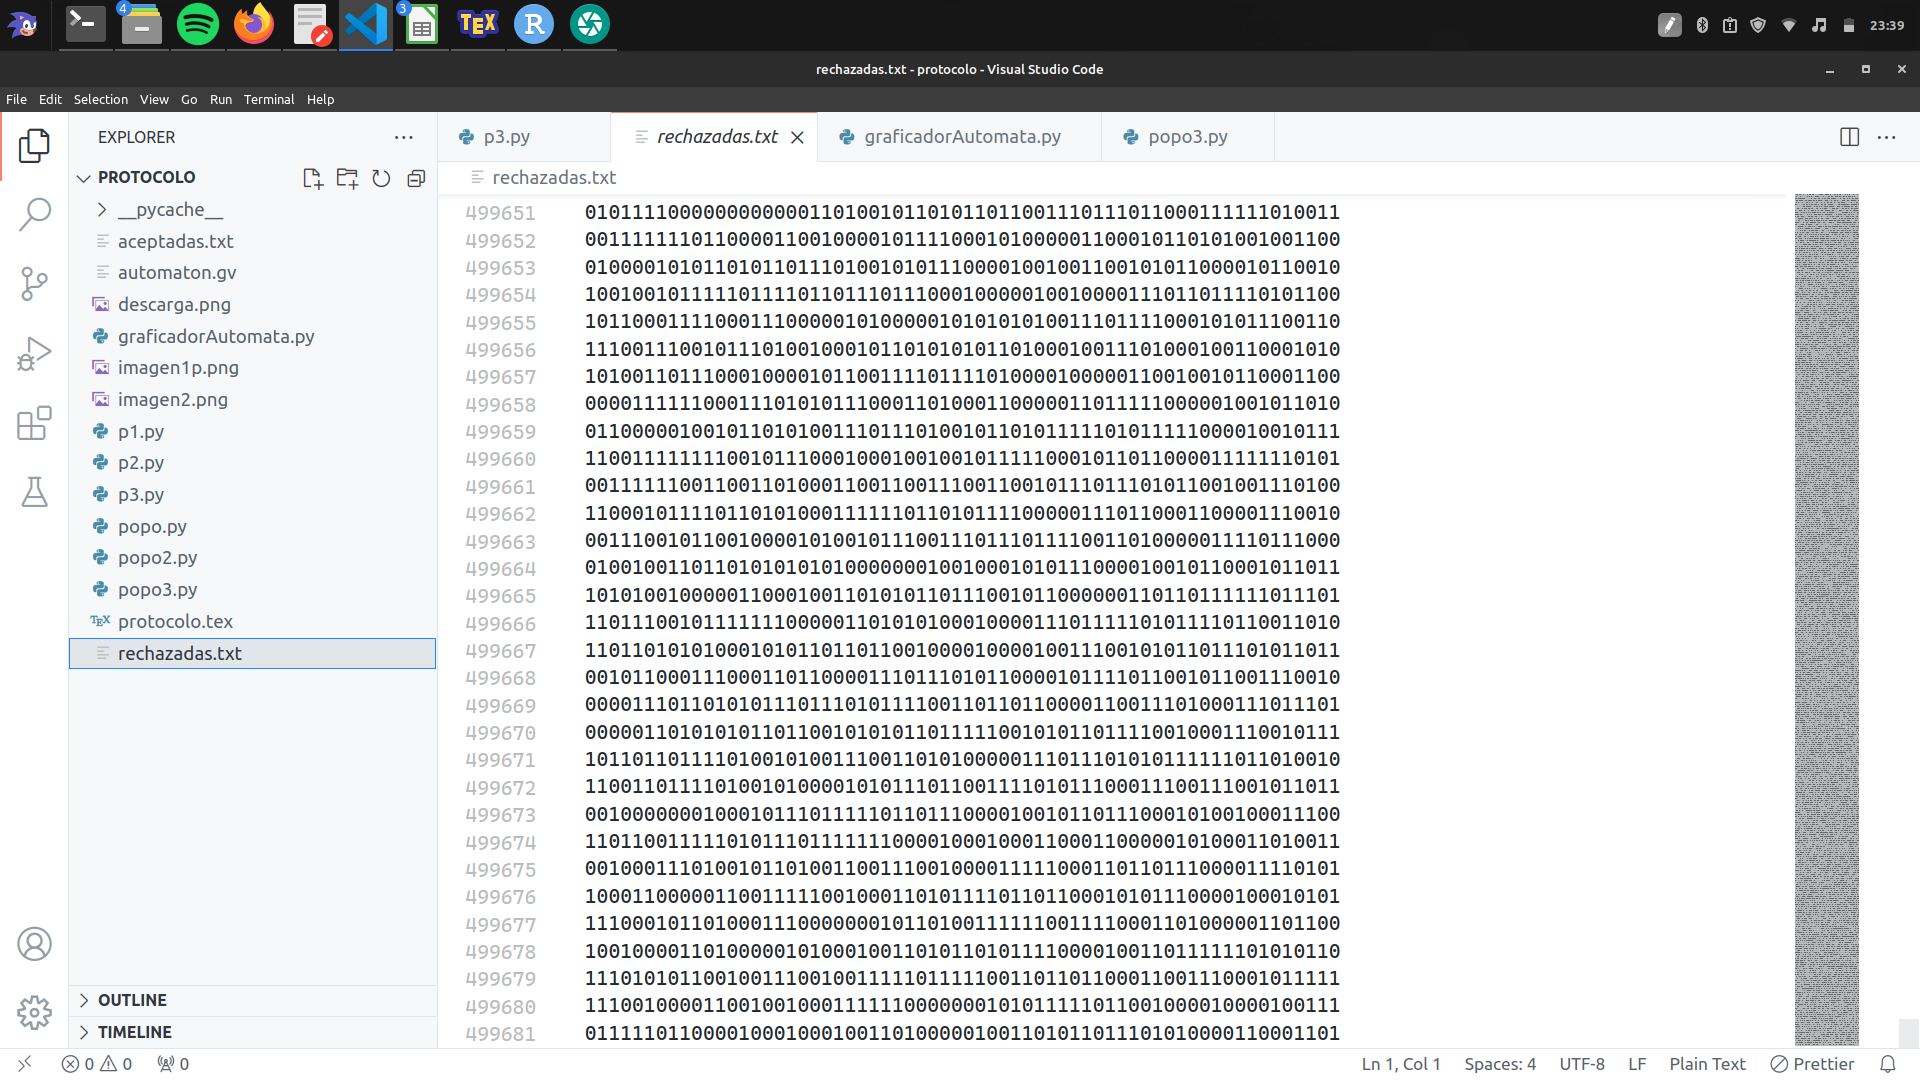
\includegraphics[width=0.8\textwidth]{hola.png}
		\caption{Archivo de rechazadas}
	\end{figure}
	
	
	\section{Código de Implementación}
	
	\subsection{Programa principal}
	
	\begin{lstlisting}
		
	'''
	INSTITUTO POLITÉCNICO NACIONAL
	ESCUELA SUPERIOR DE CÓMPUTO
	
	INGENIERÍA EN INTELIGENCIA ARTIFICIAL
	
	TEORÍA DE LA COMPUTACIÓN
	PROTOCOLO
	
	GRUPO: 5BM1
	ALUMNO: TREJO ARRIAGA RODRIGO GERARDO
	
	ESTE PROGRAMA SIMULA UN PROTOCOLO EN EL QUE CLASIFICA PALABRAS BINARIAS SEGÚN SU PARIDAD:
	
	i) GENERA PALABRAS RANDOM Y LAS CLASIFICA DEPENDIENDO SI LA CANTIDAD DE UNOS Y CEROS QUE TIENEN
	ES PAR O NO
	ii) ESCRIBE LAS PALABRAS CON UNOS Y CEROS PAR EN UN ARCHIVO DE TEXTO
	iii) GRAFICA EL AUTÓMATA DEL PROTOCOLO Y EL DE PARIDAD
	
	ÚLTIMA MODIFICACIÓN: 13/10/2023
	'''
	
	#  --------------------------------------------------------------------------------------------------------------------
	# MÓDULOS Y LIBRERÍAS IMPORTADAS
	
	
	import random
	import os
	from graficadorAutomata import *
	
	#  --------------------------------------------------------------------------------------------------------------------
	# FUNCIONES
	
	
	def eliminar_archs(nombre_arch):
	"""Función que elimina un archivo si existe en el directorio
	
	Args:
	nombre_arch (str): Nombre del archivo que deseas eliminar
	"""
	archivo1 = nombre_arch
	if os.path.exists(archivo1):
	os.remove(archivo1)
	
	
	def automata_paridad(transiciones:dict, palabra: str) -> int:
	"""Función que simula las trancisiones del autómata de paridad para evaluar una palabra
	
	Args:
	transiciones (dict): Diciionario de transiciones del autómata
	palabra (str): Palabra que se evalúa en el autómata
	
	Returns:
	int: Estado en el que se quedó la palabra
	"""
	estado = 0
	for caracter in palabra:
	estado = transiciones[(estado, caracter)]
	return estado
	
	
	def generar_palabras(num_palabras: int, long_cadena:int) -> list:
	"""Función que genera la lista de palabras binarias random
	
	Args:
	num_palabras (int): Número de palabras que tendrá la lista
	long_cadena (int): Longitud de cada palabra binaria
	
	Returns:
	list: Lista de palabras binarias
	"""
	return [''.join([str(random.randint(0, 1)) for _ in range(long_cadena)]) for _ in range(num_palabras)]
	
	
	def filtrar_palabras(palabras:list, transiciones) -> tuple:
	"""Función que filtra palabras binarias según su paridad de unos y ceros
	
	Args:
	palabras (list): Lista de palabras que se evaluarán
	transiciones (_type_): Diccionario con las transiciones del autómata
	
	Returns:
	tuple: Lista de palabras aceptadas y rechazadas por el autómata
	"""
	aceptadas = []
	rechazadas = []
	for palabra in palabras:
	if automata_paridad(transiciones, palabra) == 0:
	aceptadas.append(palabra)
	else:
	rechazadas.append(palabra)
	return aceptadas, rechazadas
	
	
	def escribir_en_archivo(nombre_arch: str, datos:list) -> None:
	"""Función que escribe una lista de palabras en un archiivo
	
	Args:
	nombre_arch (str): Nombre del archivo en el que se escribirán los datos
	datos (list): Lista de datos que se escribirán
	"""
	if datos:
	with open(nombre_arch, "a+") as archivo:
	archivo.write("\n ".join(datos))
	archivo.write("\n ")
	
	
	def graficar_estados(graficador)-> None:
	"""Función que dibuja los estados
	
	Args:
	drawer (graphic): Objeto que dibuja un autómata
	"""
	graficador.dibujar_estado(200, 150, 2.5, radio=50, flag_inicial=False, etiqueta="Ready")
	graficador.dibujar_estado(600, 150, 2.7, radio=50, flag_inicial=False, etiqueta="Sending")
	graficador.dibujar_estado(400, 300, 2.7, radio=45, flag_inicial=True, etiqueta="q0")
	graficador.dibujar_estado(200, 450, 2.7, radio=45, flag_inicial=False, etiqueta="q1")
	graficador.dibujar_estado(600, 450, 2.7, radio=45, flag_inicial=False, etiqueta="q3")
	graficador.dibujar_estado(400, 630, 2.7, radio=45, flag_inicial=False, etiqueta="q4")
	
	
	def graficar_transiciones(graficador)->None:
	"""Función quen dibuja las transiciones
	
	Args:
	drawer (graphic): Objeto que dibuja un autómata
	"""
	graficador.dibujar_transicion(250, 150, 550, 150, "data in", 15, 2, 10, -20)
	graficador.dibujar_ciclo(650, 150, radio=30, etiqueta="time_out", cte_x=17, cte_y=-37, cte_text=0.1)
	graficador.dibujar_transicion(225, 190, 358, 290, ancho_linea=2)
	graficador.dibujar_transicion(445, 290, 570, 190, ancho_linea=2)
	graficador.dibujar_transicion(232, 420, 358, 320, "1", ancho_linea=2, cte_y=-26)
	graficador.dibujar_transicion(243, 445, 372, 340, "1", ancho_linea=2, cte_y=35)
	graficador.dibujar_transicion(570, 420, 440, 315, "0", ancho_linea=2, cte_y=-26)
	graficador.dibujar_transicion(555, 445, 427, 339, "0", ancho_linea=2, cte_y=35)
	graficador.dibujar_transicion(440, 620, 575, 490, "1", ancho_linea=2, cte_y=35)
	graficador.dibujar_transicion(400, 630, 560, 470, "1", ancho_linea=2, cte_y=-26)
	graficador.dibujar_transicion(355, 630, 210, 490, "0", ancho_linea=2, cte_y=35)
	graficador.dibujar_transicion(365, 605, 235, 480, "0", ancho_linea=2, cte_y=-26)
	
	
	def graficar_uniones(graficador) ->None:
	"""Función que dinuja las uniones
	
	Args:
	drawer (graphic): Objeto que dibuja un autómata
	"""
	graficador.dibujar_circulo(545, 150, 7)
	graficador.dibujar_circulo(650, 120, 7)
	graficador.dibujar_circulo(228, 193, 7)
	graficador.dibujar_circulo(448, 287, 7)
	graficador.dibujar_circulo(355, 317, 7)
	graficador.dibujar_circulo(243, 445, 7)
	graficador.dibujar_circulo(565, 417, 7)
	graficador.dibujar_circulo(430, 340, 7)
	graficador.dibujar_circulo(445, 614, 7)
	graficador.dibujar_circulo(557, 473, 7)
	graficador.dibujar_circulo(213, 496, 7)
	graficador.dibujar_circulo(360, 600, 7)
	
	
	def graficar_protocolo():
	"""Función que genera el autómata
	"""
	graficador = AutomataDrawer(850, 800)
	graficador.colocar_titulo("Autómata de Protocolo")
	graficar_transiciones(graficador)
	graficar_uniones(graficador)
	graficar_estados(graficador)
	input("Presiona Enter para cerrar la ventana...")
	graficador.close()
	
	#  --------------------------------------------------------------------------------------------------------------------
	# FUNCIÓN PRINCIPAL MAIN
	
	
	if __name__ == "__main__":
	
	transiciones = {
		(0, '0'): 1, (0, '1'): 3,
		(1, '0'): 0, (1, '1'): 2,
		(2, '0'): 3, (2, '1'): 1,
		(3, '0'): 2, (3, '1'): 0
	}
	
	nombre_aceptadas = "aceptadas.txt"
	nombre_rechazadas = "rechazadas.txt"
	
	long_cadena = 64
	num_palabras = 1000000
	num_act = 0
	
	os.system('clear')
	print("\t\t\t***PROTOCOLO***\n")
	
	eliminar_archs(nombre_aceptadas)
	eliminar_archs(nombre_rechazadas)
	
	while random.randint(0,1):
	print("Protocolo en ejecución")
	palabras = generar_palabras(num_palabras, long_cadena)
	print("\t>> Esperando ...")
	aceptadas, rechazadas = filtrar_palabras(palabras, transiciones)
	escribir_en_archivo(nombre_aceptadas, aceptadas)
	escribir_en_archivo(nombre_rechazadas, rechazadas)
	print("Palabras clasificadas\n")
	num_act += 1
	
	if num_act != 0:
	print(f"Numero de ejecuciones del protocolo: {num_act}\n")
	print(f"Puedes consultar la clasificación de palabras en {nombre_aceptadas} & {nombre_rechazadas}")
	else:
	print("El protocolo no se ha podido ejecutar, inténtalo nuevamente.")
	
	graficar_protocolo()
	
		
	\end{lstlisting}
	
	\subsection{Graficador de Autómata}
	\begin{lstlisting}
	from graphics import *
	import math
	
	class AutomataDrawer:
	"""Clase que dibuja los elementos de un autómata de manera gráfica
	"""
	
	
	def __init__(self, ancho:int , alto: int):
	"""Constructor de la clase graficadora de autómatas
	
	Args:
	ancho (int): Ancho de la ventana donde se dibujará el autómata
	alto (int): Alto de la ventana donde se dibujará el autómata
	"""
	self.win = GraphWin("Automata Drawer", ancho, alto)
	self.states = []
	
	
	def colocar_titulo(self, titulo: str, pos: tuple =(425, 40), tam_letra: int =24) -> None:
	"""Método que añade el título del autómata
	
	Args:
	titulo (str): título que se colocará en la gráfica
	pos (tuple, optional): Coordenadas donde irá el título. Defaults to (425, 40).
	tam_letra (int, optional): tamaño del título. Defaults to 24.
	"""
	titulo = Text(Point(pos[0], pos[1]), titulo)
	titulo.setSize(tam_letra)
	titulo.setStyle("bold")
	titulo.draw(self.win)
	
	
	def dibujar_estado(self, x:int, y:int, tam_text:int, radio:int=20, flag_inicial:bool=False, etiqueta:str=None, ancho_linea:int=2) -> None:
	"""Método que dibuja un estado del autómata
	
	Args:
	x (int): Coordenada x del centro del círculo
	y (int): Coordenada y del centro del círculo
	tam_text (int): Tamaño del estado del autómata
	radio (int, optional): Radio del estado. Defaults to 20.
	flag_inicial (bool, optional): Bandera que indica si es estado inicial. Defaults to False.
	etiqueta (str, optional): Nombre del estado. Defaults to None.
	ancho_linea (int, optional): Ancho de la línea del círculo. Defaults to 2.
	"""
	estado = Circle(Point(x, y), radio)
	estado.setWidth(ancho_linea)
	estado.setFill("green")
	estado.setOutline("blue")
	estado.draw(self.win)
	
	if flag_inicial:
	circulo_ini = Circle(Point(x, y), radio - 5)
	circulo_ini.setFill("white")
	circulo_ini.draw(self.win)
	
	if etiqueta:
	text = Text(Point(x, y), etiqueta)
	text.setSize(int(radio / tam_text))
	text.draw(self.win)
	
	self.states.append(estado)
	
	
	def dibujar_transicion(self, x1:int, y1:int, x2:int, y2:int, etiqueta:str=None, tam_text:int=12, ancho_linea:int=2, cte_x:int=0, cte_y:int=0) -> None:
	"""Método que dinuja la linea de transición entre estados
	
	Args:
	x1 (int): Posicion inicial en x de la línea
	y1 (int): Posicion inicial en y de la línea
	x2 (int): Posicion final en x de la línea
	y2 (int): Posicion final en y de la línea
	etiqueta (str, optional): Etiqueta de la transición. Defaults to None.
	tam_text (int, optional): Tamaño de la etiqueta. Defaults to 12.
	ancho_linea (int, optional): Ancho de la etiqueta. Defaults to 2.
	cte_x (int, optional): Desplazamiento en x de la etiqueta con respecto al centro de la linea. Defaults to 0.
	cte_y (int, optional): Desplazamiento en y de la etiqueta con respecto al centro de la linea. Defaults to 0.
	"""
	linea = Line(Point(x1, y1), Point(x2, y2))
	linea.setOutline("black")
	linea.setWidth(ancho_linea) 
	linea.draw(self.win)
	
	if etiqueta:
	x = (x1 + x2 +cte_x) / 2
	y = (y1 + y2 +cte_y) / 2
	text = Text(Point(x, y), etiqueta)
	text.setSize(tam_text)
	text.draw(self.win)
	
	
	def dibujar_circulo(self, x:int, y:int, radius:int, color:str="darkblue")->None:
	"""Dibuja un círculo para simular 'la llegada' de una transición
	
	Args:
	x (int): Coordenada en x del centro del cículo
	y (int): Coordenada en y del centro del cículo
	radius (int): Radio del círculo
	color (str, optional): Color del círculo. Defaults to "darkblue".
	"""
	circulo = Circle(Point(x, y), radius)
	circulo.setFill(color)
	circulo.setOutline(color)
	circulo.draw(self.win)
	
	
	def dibujar_ciclo(self, x:int, y:int, radio:int=20, etiqueta:str=None, flag_hor:bool=False, cte_x:int=0, cte_y:int=0, cte_text:int=0, grosor_linea:int=2)-> None:
	"""Método que simula la transición al mismo estado mediante un semicírculo
	
	Args:
	x (int): Coordenada en x del centro del semicírculo
	y (int): Coordenada en x del centro del semicírculo
	radio (int, optional): Radio del semincírculo. Defaults to 20.
	etiqueta (str, optional): Etiqueta de la transición. Defaults to None.
	flag_hor (bool, optional): Bandera de si el semicírculo será horizontal. Defaults to False.
	cte_x (int, optional): Desplazamiento en x de la etiqueta con respecto al centro del semicirculo. Defaults to 0.
	cte_y (int, optional): Desplazamiento en y de la etiqueta con respecto al centro del semicirculo. Defaults to 0.
	cte_text (int, optional): Ajusta el tamaño del texto. Defaults to 0.
	grosor_linea (int, optional): Grosor de la línea de transición. Defaults to 2.
	"""
	num_segments = 20
	if flag_hor:
	angulo_ini = 0
	end_angle = 180
	else:
	angulo_ini = -90
	end_angle = 90
	incremento = (end_angle - angulo_ini) / num_segments
	
	for i in range(num_segments + 1):
	angulo = angulo_ini + i * incremento
	x1 = x + radio * math.cos(math.radians(angulo))
	y1 = y + radio * math.sin(math.radians(angulo))
	angulo += incremento
	x2 = x + radio * math.cos(math.radians(angulo))
	y2 = y + radio * math.sin(math.radians(angulo))
	line = Line(Point(x1, y1), Point(x2, y2))
	line.setWidth(grosor_linea)
	line.setOutline("black")
	line.draw(self.win)
	
	if etiqueta:
	if flag_hor:
	text = Text(Point(x+cte_x, y+cte_y), etiqueta)
	text.setSize(int(radio / 2+cte_text))
	text.draw(self.win)
	else:
	text = Text(Point(x+cte_x, y+cte_y - radio * 0.5), etiqueta)
	text.setSize(int(radio / 2+cte_text))
	text.draw(self.win)
	
	
	def clear(self)-> None:
	"""Método que borra todos los elementos dibujados en la ventana
	"""
	for state in self.states:
	state.undraw()
	self.states = []
	self.win.update()
	
	
	def close(self):
	"""Método que cierra la ventana de la gráfica
	"""
	self.win.close()
	
	\end{lstlisting}
	
	
	
\end{document}